\documentclass[twoside,12pt]{article}
\usepackage[left=1in, right=1in, top=1in, bottom=1in]{geometry}
\usepackage{amsmath}
\usepackage{amssymb}
\usepackage{amsfonts}
\usepackage{mathtools}
\usepackage{amsthm}
\usepackage{fancyhdr}
\usepackage{enumitem}
\usepackage{siunitx}
\usepackage{booktabs}
\usepackage[hidelinks]{hyperref}
\usepackage{sectsty}
\usepackage{mathrsfs} % mathscr
\usepackage{tikz}
\usepackage{pgfplots}
\usepackage{multicol}
\usepackage{listings}
% \usepackage{amsart}
\usepackage{fontspec}
\usepackage{titlesec}

% allow H option of figure
\usepackage{float}

% math font (libertine)
\usepackage{libertinus-otf}

% braket
\usepackage{braket}

% mono font
\usepackage{inconsolata}
\setmonofont{inconsolata}

% define latin modern font environment
\newcommand{\lms}{\fontfamily{lmss}\selectfont} % Latin Modern Roman
% \newcommand{\lmss}{\fontfamily{lmss}\selectfont} % Latin Modern Sans
% \newcommand{\lmss}{\fontfamily{lmtt}\selectfont} % Latin Modern Mono

% % change mathcal shape
% \usepackage[mathcal]{eucal}


% define math operators
\newcommand{\FF}{\mathbb{F}}
\newcommand{\RR}{\mathbb{R}}
\newcommand{\NN}{\mathbb{N}}
\newcommand{\ZZ}{\mathbb{Z}}
\newcommand{\QQ}{\mathbb{Q}}
\newcommand{\XX}{\mathbb{Y}}
\newcommand{\CL}{\mathcal{L}}
% \renewcommand{\d}{\mathrm{d}}
\renewcommand*\d{\mathop{}\!\mathrm{d}}
\DeclareMathOperator*{\argmax}{arg\,max}
\DeclareMathOperator*{\argmin}{arg\,min}
\DeclareMathOperator{\im}{im}
\DeclareMathOperator{\id}{id}
\renewcommand{\mod}[1]{\ (\mathrm{mod}\ #1)}

% section font style
\sectionfont{\lms\large}
\subsectionfont{\lms\normalsize}
\subsubsectionfont{\bf}

% line spreading and break
\hyphenpenalty=5000
\tolerance=20
\setlength{\parindent}{0em}
\setlength\parskip{0.5em}
\allowdisplaybreaks
\linespread{0.9}

% theorem
% latex theorem
% definition style
\theoremstyle{definition}
\newtheorem{theorem}{Theorem}[subsection]
\newtheorem{axiom}{Axiom}[section]
\newtheorem{definition}{Definition}[section]
\newtheorem{example}{Example}[section]
\newtheorem{question}{Question}[section]
\newtheorem{exercise}{Exercise}[section]
\newtheorem*{exercise*}{Exercise}
\newtheorem{lemma}{Lemma}[section]
\newtheorem{proposition}{Proposition}[section]
\newtheorem{corollary}{Corollary}[section]
\newtheorem*{theorem*}{Theorem}
\newtheorem{problem}{Problem}
% remark style
\theoremstyle{remark}
\newtheorem*{remark}{Remark}
\newtheorem*{solution}{Solution}
\newtheorem*{claim}{Claim}


% paragraph indent
\setlength{\parindent}{0em}
\setlength\parskip{0.5em}

\newcommand\Code{CSC4005 FA22}
\newcommand\Ass{HW01}
\newcommand\name{Haoran Sun}
\newcommand\mail{haoransun@link.cuhk.edu.cn}

\title{{\lms \Code \ \Ass}}
\author{\lms \name \ (\href{mailto:\mail}{\mail})}
\date{\sffamily \today}

\makeatletter
% \let\Title\@title
\let\theauthor\@author
\let\thedate\@date

\fancypagestyle{plain}{%
    \fancyhf{}
    \lhead{\sffamily \Ass}
    \rhead{\sffamily \name}
    \rfoot{\sffamily\thepage}

    % # 页脚自定义
    \fancyfoot[L]{
        \begin{minipage}[c]{0.06\textwidth}
            
\includegraphics[height=7.5mm]{logo2.png}
        \end{minipage}
    }
}
\fancypagestyle{title}{%
    \fancyhf{}
    \renewcommand{\headrulewidth}{0pt}
    % \lhead{\Title}
    % \rhead{\theauthor}
    \rfoot{\sffamily\thepage}

    % # 页脚自定义
    \fancyfoot[L]{
        \begin{minipage}[c]{0.06\textwidth}
            
\includegraphics[height=7.5mm]{logo2.png}
        \end{minipage}
    }
}
\fancyfootoffset[L]{0.3cm}

% re-define title format
\makeatletter
\renewcommand{\maketitle}{\bgroup\setlength{\parindent}{0pt}
\begin{flushleft}
  \textbf{\Large\@title}

  \@author
\end{flushleft}\egroup
}
\makeatother

\pagestyle{plain}

% lstlisting settings
\lstset{
    basicstyle=\linespread{0.8}\ttfamily\small,
    breaklines=true,
    basewidth=0.5em,
    frame=single,
}
\lstdefinestyle{output}{
    basicstyle=\ttfamily\small,
}    
\lstdefinestyle{cpp}{
    numbers=left,
    basicstyle=\linespread{0.8}\ttfamily\small,
    numberstyle=\linespread{0.8}\ttfamily\small,
    language=C++,
    xleftmargin=6.0ex,
    frame=single,
}


\begin{document}
\maketitle
\thispagestyle{title}

\section{Introduction}
Similar to bubble sort, the odd-even sort is a sorting algorithm with complexity $O(n^2)$.
In this assignment, the MPI library was utilized to improve the
sorting speed with the benefit of multi-processing.
A sequential and a parallel version of the sorting algorithm were implemented.
The program was tested under different array sizes and numbers of CPU cores.
The speed-up factor and CPU efficiency were also analyzed.



\section{Method}
\subsection{Program design and implementation}
The sequential and parallel sorting programs were implemented using the C++ programming language.
MPICH library was used for the parallel part.
The parallel version was written in \lstinline|src/main.cpp|, 
while the sequential version was written in \lstinline|src/main.seq.cpp|.
Some important functions were written in \lstinline|src/utils.h|.

For the flowchart, please refer to Figure \ref{fig:flowchart}.
The sequential sorting function is printed as the following c++ function.
\begin{lstlisting}[style=cpp]
// binary sort
void odd_even_sort(int* arr, int N, int f){
    if (f==1) return;
    int a, b;
    int flag = 1;
    // odd loop
    for (int i = 1; i < N; i += 2){
        a = arr[i-1];
        b = arr[i];
        if (b < a){
            arr[i]   = a;
            arr[i-1] = b;
            flag = 0;
        }
    }
    // even loop
    for (int i = 2; i < N; i += 2){
        a = arr[i-1];
        b = arr[i];
        if (b < a){
            arr[i]   = a;
            arr[i-1] = b;
            flag = 0;
        }
    }
    return odd_even_sort(arr, N, flag);
}
\end{lstlisting}
The parallel sorting scheme is similar.
However, when the odd-even comparison involves numbers in two processes,
\lstinline|MPI_Sendrecv| were called.
For example, the following code performs the edge case by calling
\lstinline|MPI_Sendrecv()|.
\begin{lstlisting}[style=cpp]
if (start_idx>0 && start_idx%2==1){
    // printf("odd start_idx %d rank %d sendrecv rank %d\n", start_idx, rank, rank-1);
    to = arr[0];
    MPI_Sendrecv(&to, 1, MPI_INT, rank-1, 1, &from, 1, MPI_INT, rank-1, 2, MPI_COMM_WORLD, MPI_STATUS_IGNORE);
    if (from > to) {
        arr[0] = from;
        flag = 0;
    }
} 
else if ((end_idx-1)%2==0 && end_idx<N){
    // printf("odd end_idx %d rank %d sendrecv rank %d\n", end_idx, rank, rank+1);
    to = arr[end_idx-start_idx-1];
    MPI_Sendrecv(&to, 1, MPI_INT, rank+1, 2, &from, 1, MPI_INT, rank+1, 1, MPI_COMM_WORLD, MPI_STATUS_IGNORE);
    if (from < to) {
        arr[end_idx-start_idx-1] = from;
        flag = 0;
    }
}
\end{lstlisting}

The program is compiled using CMake build system.
One can have a look in \lstinline|CMakeLists.txt| and \lstinline|src/CMakeLists.txt| 
to check compilation requirements.
If one wants to build the program, he can run the following commands to
configure and start compilation under \lstinline|hw01| directory.
The compiled programs are placed in \lstinline|build/bin| directory.
\begin{lstlisting}
cmake -B build -DCMAKE_BUILD_TYPE=Release # write configure files in ./build
cmake --build build                       # build the program in ./build
\end{lstlisting}
After the building process is finished, for example,
one can run the program using the following commands.
\begin{lstlisting}
./build/bin/main.seq -n 20 --save 0 --print 1           # sequential program
mpirun -np 10 ./build/bin/main -n 20 --save 0 --print 1 # parallel program 
\end{lstlisting}
\lstinline|-n 10| means set array size to 10, \lstinline|--save 0|
means do not save any runtime data, and \lstinline|--print 1|
means output the randomly generated array at first and output
the sorted array at the end.


\subsection{Performance evaluation}
In order to evaluate the parallel code, the program was executed under 
different configurations.
With 20 different CPU core numbers (from 4 to 80 with increment 4, $n=4, 8,\dots, 80$)
and 20 different array sizes (from 50000 to 1000000 with increment 50000, $N=50000, 100000, \dots, 1000000$), 
overall, 400 cases were sampled.
Recorded runtime and CPU time were analyzed through the Numpy package in Python.
Figures were plotted through the Matplotlib and the Seaborn packages in Python.
Analysis code were written in \lstinline|analysis/main.ipynb|.
It is highly recommended to set \lstinline|--print 0| when the array size is large.


\newpage
\section{Result and Discussion}
\subsection{Running time}
\begin{figure}[H]
    \centering
    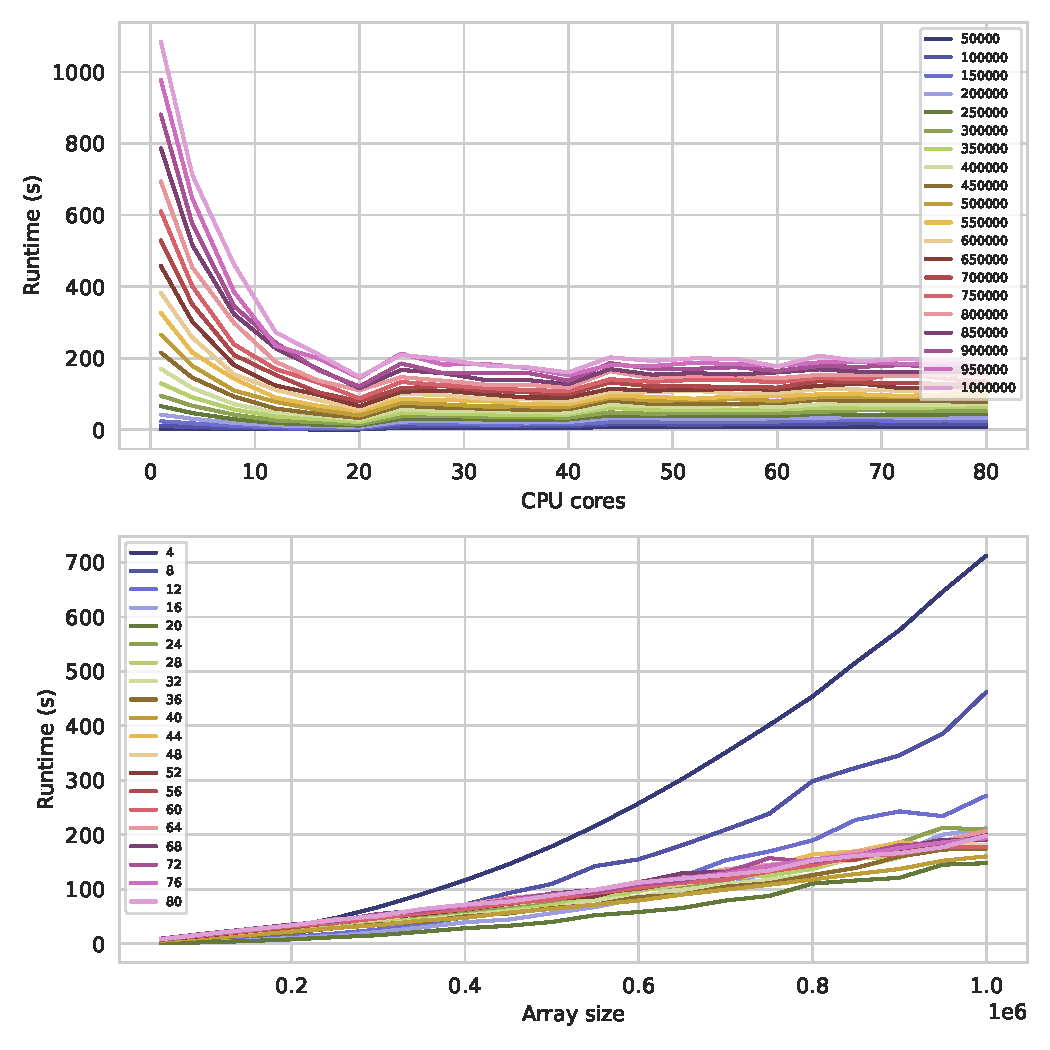
\includegraphics[width=\textwidth]{../analysis/runtime.pdf}
    \caption{Running time versus the number of CPU cores}
    \label{fig:runtime}
\end{figure}

The graph of running time versus CPU cores and versus array size were plotted
in Figure \ref{fig:runtime}.
From this figure, we can see that when the array size is small,
the parallelism will not make the program faster but will slow down the execution time.
However, when the array size is large enough (e.g., 150000), we can observe a strong
speed-up effect if we use more than one core.
From Figure \ref{fig:runtime}, we can observe an obvious $O(n^2)$ complexity
of the algorithm.
It also should be noted that in the case of a large array,
with the increase in CPU cores,
the running time keeps dropping until the number of cores exceeds 20.


\subsection{Performance analysis}
\begin{figure}[H]
    \centering
    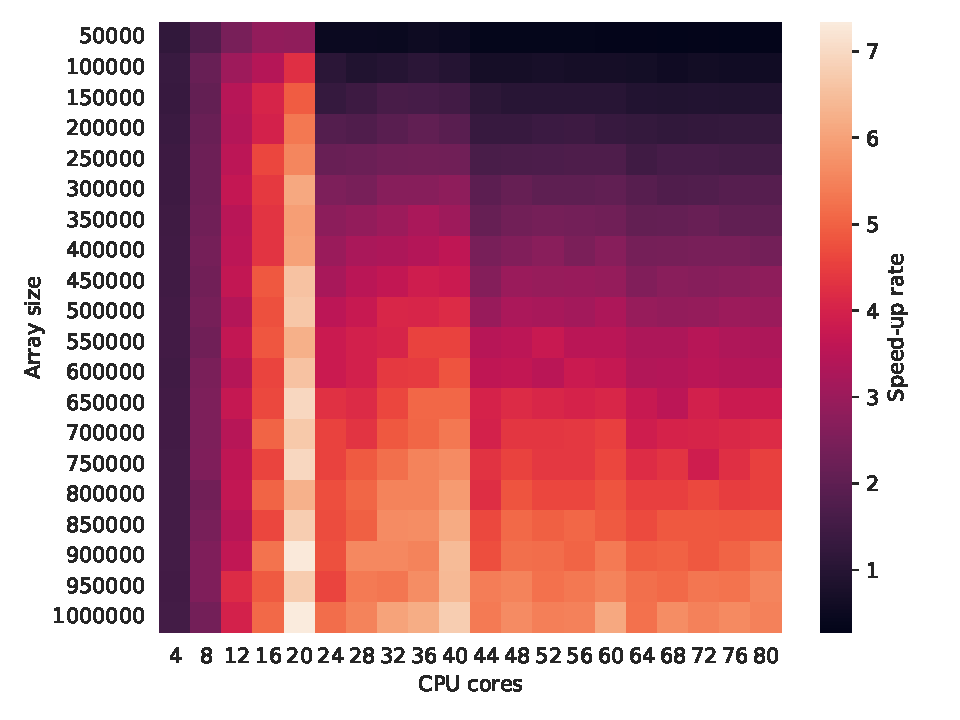
\includegraphics[width=\textwidth]{../analysis/rate_heatmap.pdf}
    \caption{Heatmap of speed-up rate}
    \label{fig:rate-heat}
\end{figure}
The speed-up rate is defined as the following ratio, where $N$ denotes the array size
and $n$ is the CPU core numbers in a parallel program.
\begin{align}
    r(N, n) = \frac{\text{runtime of sequential sorting a size $N$ array}}
    {\text{runtime of parallel sorting a size $N$ array using $n$ processes}}
\end{align}
Therefore, we can calculate a speed-up rate for each sample $(N, n)$.
The heatmap of the speed-up rate is plotted in Figure \ref{fig:rate-heat}.
A 3D version of the heatmap is also provided in Figure \ref{fig:rate-heat3d} for better visualization.
The speed-up rate versus array size and CPU core number is plotted in Figure \ref{fig:rate}.

\begin{figure}[H]
    \centering
    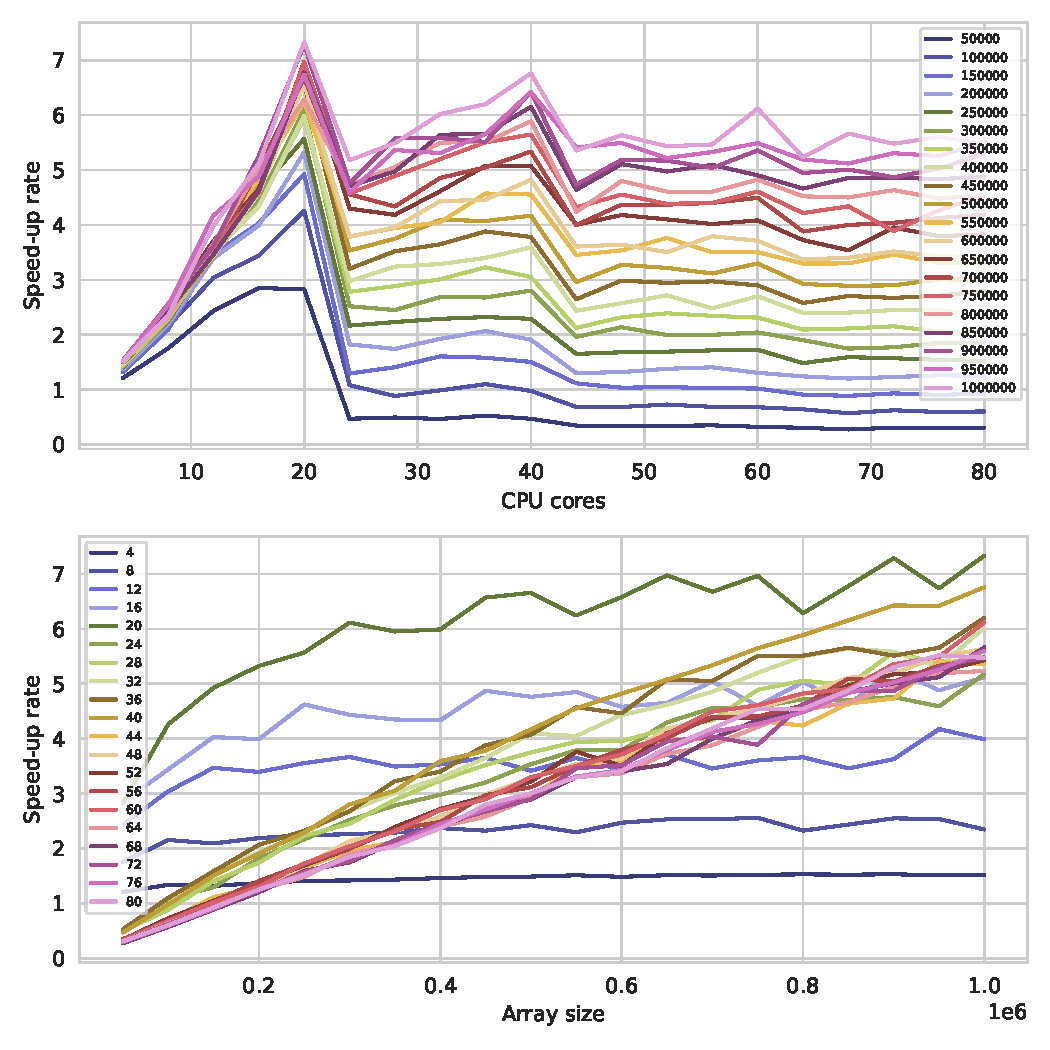
\includegraphics[width=\textwidth]{../analysis/rate.pdf}
    \caption{Speed up rate versus the number of CPU cores and array size}
    \label{fig:rate}
\end{figure}

Noticeably, the maximum speed-up rate was achieved in $N=1000000$ and $n=20$.
Interestingly, in Figure \ref{fig:rate}, for a fixed array size,
the speed-up rate will have a significant drop if the CPU core number just exceeds 20, 40, and 60.
The reason for this could be highly caused by the configuration of the cluster.
In the CSC4005 computing cluster, it is easy to discover that each node contains
20 CPU cores.
If the CPU cores exceed 20, the program would involve more than one node.
Obviously, the primary influence of multi-node computing would be communication latency.
Since MPI is not designed for the shared memory system, data must be transferred during the
calculation.
Therefore, we can deduct the conclusion that the optimal MPI configuration
under this cluster would be 20 cores.
Moreover, speculation could be proposed that the optimal MPI configuration
for any cluster is one node with all its available CPU cores.


Also, according to the plot of speed-up rate versus array size in Figure \ref{fig:rate},
we can see that if we only use one computing node, the speed-up rate is not
significantly affected by the array size.
However, as long as the calculation involves two or more nodes, the speed-up rate 
dropped notably when the array size is relatively small.
Also, the speed-up rate is no longer sensitive to the increment of total CPU cores
used in sorting.
That is because when the array size becomes large, the latency caused by
the odd-even transition would be less dominant.


\section{Conclusion}
In conclusion, a parallel odd-even sorting algorithm was implemented and
its performance was evaluated.
When the array size is small, the sequential program is more efficient.
While the parallel program is more efficient when the array size
is large.
However, it is better not to use more than one node since the latency
caused by inter-node communication could significantly increase the
runtime.



\newpage
\appendix
% \renewcommand\thefigure{\thesection.\arabic{figure}}
\counterwithin{figure}{section}

\newpage
\section{Supplementary figures}
\begin{figure}[H]
    \centering
    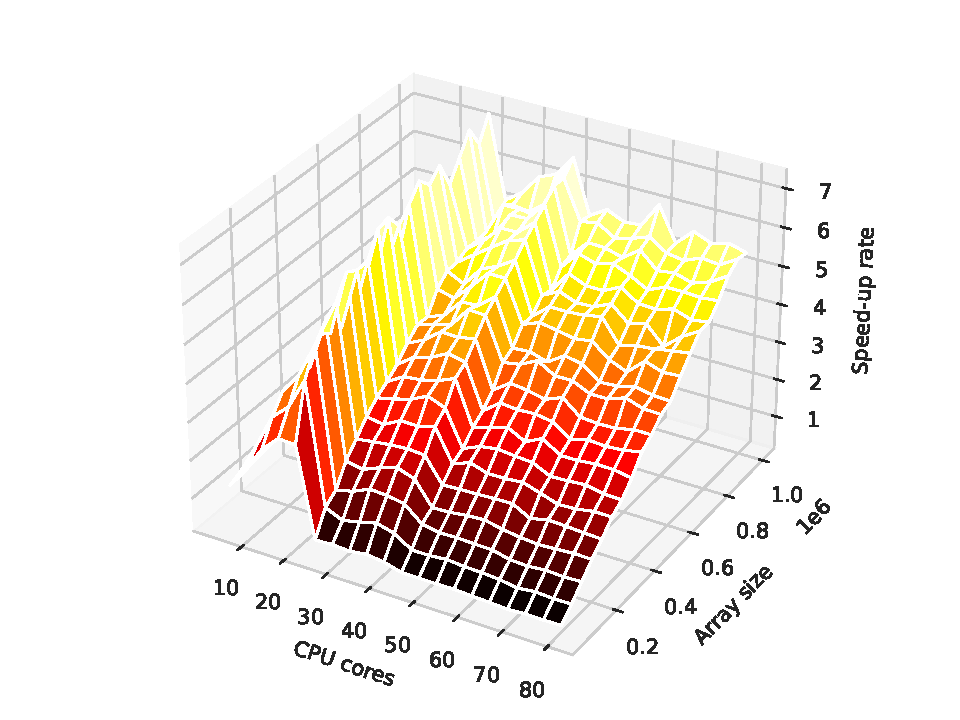
\includegraphics[width=0.75\textwidth]{../analysis/rate_heatmap_3d.pdf}
    \caption{3D heatmap of speed-up rate}
    \label{fig:rate-heat3d}
\end{figure}
\begin{figure}[H]
    \centering
    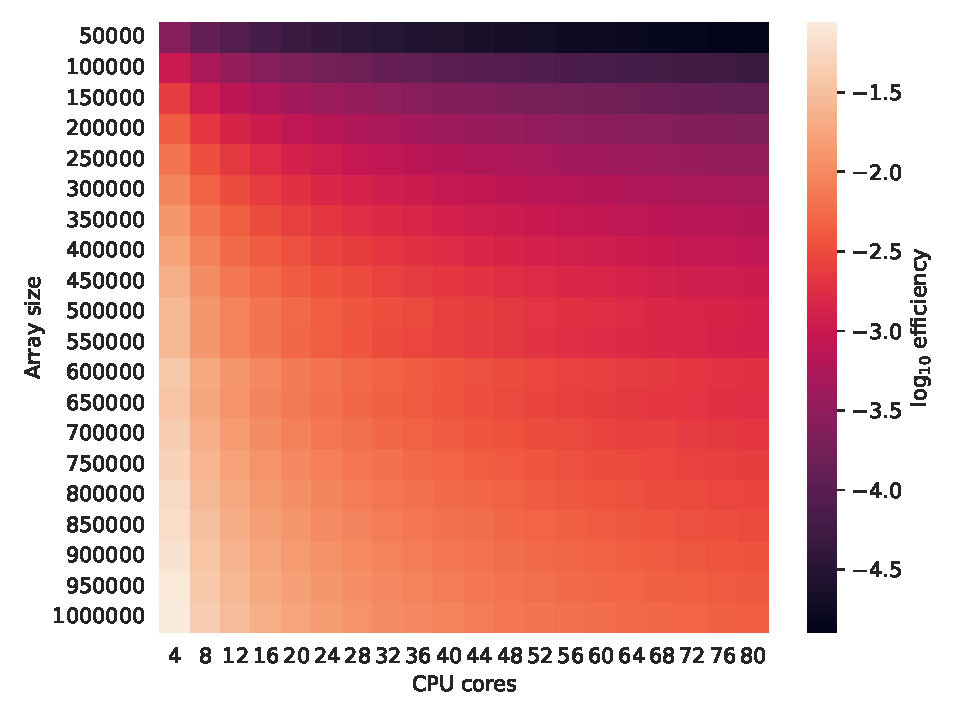
\includegraphics[width=0.75\textwidth]{../analysis/logeff_heatmap.pdf}
    \caption{Heat map of $\log_{10} (\text{seq CPU time}/\text{par CPU time})$ }
    \label{fig:logeff}
\end{figure}

\newpage
\begin{figure}[H]
    \centering
    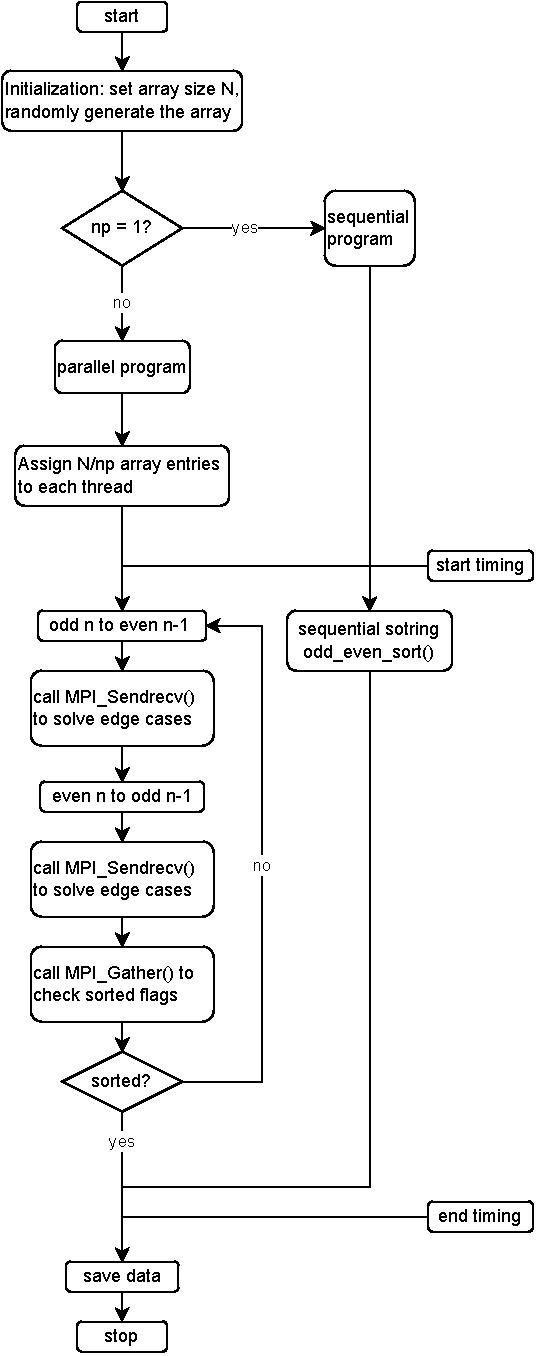
\includegraphics[height=0.95\textheight]{../flowchart_chopped.pdf}
    \caption{Program flowchart}
    \label{fig:flowchart}
\end{figure}

\newpage
\section{Source code}
\lstinputlisting[style=cpp,title=\lstinline|main.cpp|]{../src/main.cpp}
\lstinputlisting[style=cpp,title=\lstinline|main.seq.cpp|]{../src/main.seq.cpp}
\lstinputlisting[style=cpp,title=\lstinline|utils.h|]{../src/utils.h}





% \end{multicols*}
\end{document}

